\chapter{多虚拟化集群管理系统的设计}
\label{cha:multi-hypervisor-management-system}

通过努力使得 Tsinghua NOVA 系统通过 libvirt 支持了 LXC 虚拟容器,从而从单一的 QEMU-KVM
虚拟集群管理,转变为支持多种虚拟化方案的多虚拟化集群管理系统。而且,管理通过不同的虚拟化技术
运行的虚拟机的用户接口部分是完全相同的,也就是说,用户可以通过一个统一的控制面板 (control
panel) 和相同的操作方式管理由 QEMU-KVM 或是虚拟容器运行的虚拟机。

\section{容器的自动部署}
\label{sec:auto-deployment}

所谓自动部署,无论是对何种虚拟化技术,都是指的从展开客户机需要的操作系统磁盘镜像、到部署客户机的
用户态应用程序、再到连接到管理程序的虚拟机驱动并实现用户对客户机的管理的步骤。在 Tsinghua NOVA
系统中,下层的虚拟化平台对用户来讲是完全透明的。

\subsection{存储方案的比较}
\label{subsec:comparison-network-storage}

既然是一个虚拟化管理平台,那么就需要对虚拟机磁盘镜像或者根文件系统 (rootfs) 进行统一的管理。
在 Tsinghua NOVA 系统中,是由一个主节点 (master node) 提供 web 服务和虚拟机调度服务,
在多个从节点 (slave node) 上部署虚拟集群,所以这个镜像存储服务自然也是将主节点作为服务器、
从节点作为客户端的。

\subsubsection{存储的内容}

首先看一下 QEMU-KVM 的镜像文件和 LXC 的根文件系统 (rootfs) 都具有什么特点。

我们在 ~\ref{subsubsec:hardware-virt} 小节提到,QEMU-KVM 模拟设备,比如磁盘设备,
使用的是 QEMU ,因此 QEMU-KVM 支持的磁盘镜像格式就是 QEMU 支持的磁盘镜像格式,主要
包括以下几种~\cite{docker-in-practice}:

\begin{itemize}
    \item \textbf{raw:} 简单的二进制镜像,在有的文件系统,比如 xfs 和 ext4 上支持稀疏
    存储的特性,也就是分配的空间会以 metadata 的形式被记录,从而实际占用的空间小于或者等于
    分配的空间;
    \item \textbf{cow:} 简单的写时复制 (copy-on-write) 镜像,这种格式不支持 Windows
    虚拟机;
    \item \textbf{qcow:} QEMU 写时复制 (copy-on-write) 格式,已经被 \textbf{qcow2}
    格式取代了,QEMU 仍然兼容这种格式;
    \item \textbf{qcow2:} 支持快照 (snapshot) 、稀疏存储(即使在不支持上文提到的稀疏
    存储特性的文件系统上也可以实现,不受制于文件系统)、加密、压缩等高级特性的 QEMU 镜像
    格式。这种格式有很好的特性和功能表现,所以是被 Tsinghua NOVA 系统采用用来运行 KVM
    客户虚拟机操作系统的格式;
    \item \textbf{vmdk:} VMWare 的磁盘镜像格式;
    \item \textbf{vdi:} VirtualBox 的磁盘镜像格式;
\end{itemize}

QEMU 对镜像文件的格式支持非常丰富,还有几种不常用的,因为篇幅所限不能一一介绍。Tsinghua NOVA
使用 qcow2 格式,它能通过 QEMU 提供的用户态工具 qemu-img 支持虚拟机增量镜像,从而减少
网络文件系统对镜像存储的负担。因为只要存储一个操作系统的基准镜像,然后每个客户虚拟机创建
自己的增量镜像就可以了。下面简单介绍一下 qemu-img 的常见命令~\cite{docker-in-practice}。

创建一个大小为 20GB 、格式为 qcow2 的镜像文件:

\begin{lstlisting}[language=bash]
qemu-img create hello.qcow2 -f qcow2 20G
\end{lstlisting}

查看镜像的详细信息:

\begin{lstlisting}
qemu-img info hello.qcow2
\end{lstlisting}

对镜像进行格式转换,例如把 raw 格式的镜像转为 qcow2 格式的镜像(从而利用 qcow2 格式更好的
特性):

\begin{lstlisting}[language=bash]
qemu-img convert -p -f raw -O qcow2 hello hello2.qcow2
\end{lstlisting}

加上 -p 参数就可以显示进度。

对镜像进行压缩和加密,不过只有 qcow2 格式的镜像才支持这个功能,例如对刚才创建的镜像:

\begin{lstlisting}[language=bash]
qemu-img convert -c -f qcow2 -O qcow2 hello.qcow2 hello3.qcow2
qemu-img convert -f qcow2 -O qcow2 hello.qcow2 hello4.qcow2 -o encryption
\end{lstlisting}

对镜像进行快照,这也是 qcow2 格式的一个特性。例如创建一个 hello.qcow2 的快照:

\begin{lstlisting}[language=bash]
qemu-img snapshot hello.qcow2 -c snapshot00
\end{lstlisting}

创建差量镜像。之所以要使用镜像差量技术,主要是有两个好处:

\begin{enumerate}
    \item \textbf{节约时间:} 通过一个命令可以立即从基镜像生成虚拟机用到的镜像,非常快;
    \item \textbf{节约空间:} 镜像使用写时复制 (copy-on-write) 的模式,读取的时候读取
    自己的或者是基镜像的镜像文件,写入的时候才写入自己的镜像文件,也就是差量镜像,这样
    多个客户虚拟机用一个基镜像,把它们共同的点统一储存,而且只存一份,可以节约空间。
    尤其是对于 Tsinghua NOVA 这种使用网络文件系统的平台,非常重要。
\end{enumerate}

创建的方法:

\begin{lstlisting}[language=bash]
qemu-img create -f qcow2 -b hello.qcow2 hello-bak
\end{lstlisting}

使用 qemu-img 工具还可以很方便地将差量镜像整合回完整的镜像。

LXC 的根文件系统完全是在宿主的文件系统上创建的一个普通的目录,包含客户机的完整的根文件系统,
默认在 /var/lib/lxc 下。由于 namespace 技术将不同容器使用的磁盘资源做了隔离,所以不同
容器可以挂载各自的根文件系统 (rootfs) 并读写之,不会产生干扰。在宿主机上也可以直接对
这些目录进行修改,例如创建文件。

这样的好处是 LXC 的根文件系统 (rootfs) 具有可移动性 (portability) ,比如可以将一个虚拟
容器的文件系统直接拷贝到新的宿主上直接运行,可以保留原先的所有资料不至于丢失。而且在宿主上
可以直接访问客户机的根文件系统,就像一个普通目录一样,这也是一个非常方便的特性。

LXC 的用户态工具提供了一些处理根文件系统 (rootfs) 的手段,但是较为简单和直接,举例如下:

在 /var/lib/lxc/test-fedora-1/rootfs 里创建一个基于 Fedora 22 的根文件系统,
因为需要联网下载所需文件,所以速度主要取决于网速,当然宿主的磁盘 I/O 也是很重要的:

\begin{lstlisting}
lxc-create -n test-fedora-1 -t fedora
\end{lstlisting}

对根文件系统进行快照。所谓的快照就是把根文件系统 (rootfs) 复制一份保留下来:

\begin{lstlisting}
lxc-snapshot -n test-fedora-1
\end{lstlisting}

还有诸如 lxc-clone 等几个功能,总而言之是非常简单的,不仅相比 QEMU-KVM 的镜像组织
\footnote{qcow2 的镜像差量功能相当于自带了一个简单的去冗余}来说,而且相比 docker
完整的镜像定义、组织和类似 git 的版本管理也逊色很多。但是 LXC 的好处是它的基本功能
都比较简单,而且相应的 libvirt 驱动处于一个基本可用的状态,所以 Tsinghua NOVA
系统还是选取 LXC 而不是 docker 作为 Linux 虚拟容器的解决方案。当然,docker 的
“一揽子”用户态工具是非常非常方便的,类似的基于 web 的图形管理控制面板也有不少。
\footnote{比如:https://shipyard-project.com/}

\subsubsection{几种网络存储方案的选型}
\label{subsubsec:network-storage}

明确了要存储什么样的镜像资料之后,就要开始对网络存储方案进行选型。网络存储主要是为了
在创建虚拟机的时候能及时调用相应的镜像文件,从而创建并运行新的客户机。主要考察了
SSHFS / SMB / NFS 几种网络文件存储协议和文件系统。

SSHFS 的优点是它基于 FUSE 。FUSE 是一种用户态文件系统框架,可以很方便地创造用户态
文件系统。文件系统跑在用户态的好处是即使它崩掉了也不会影响系统内核的运行,比如我们
需要一个可以将云盘挂载到本地的文件系统,那么最好让它跑在用户态,因为这个功能对于操作系统
内核来讲通常是无关紧要的,即使崩溃了也没关系。基于 FUSE 文件系统的一个例子是笔者
写的 sdbfs \footnote{Simple database file system:
https://github.com/cty12/sdbfs} ,它能将文件系统的读写自动转化为 sqlite 的数据库操作。

SSHFS 的缺点也很明显,就是它是基于 SSH (secure shell) 的,创建文件只能创建使用该账户
连接的那个用户所有的,而且在一个连接内不能方便地切换用户。对于我们的需求,这个特点显得
不够灵活。而且 Tsinghua NOVA 系统因为历史遗留原因需要 root 权限运行。

SMB (Server Message Block) 是微软 Windows 系统默认使用的一种文件共享协议,可以方便
地启动“共享文件夹”\footnote{“目录” (directory) 在微软的操作系统下称为“文件夹” (folder)}
功能。SMB 服务有开源的实现叫做 samba ,被主流的 GNU/Linux 发行版包括在软件源内,但是
微软的闭源(私有)实现和 samba 的开源实现有一定的差距,而且这个差距会反映在两者的性能上。
而且 samba 的实现在小文件的读写上,和 NFS 具有一定的差距\footnote{https://
ferhatakgun.com/network-share-performance-differences-between-nfs-smb/}。

NFS (Network File System) 是一种完全开放的分布式文件系统标准,支持大多数平台,而且性能
也相对比较好。在 Tsinghua NOVA 系统中,我们使用它完成客户机操作系统镜像的共享和存储。

\subsection{虚拟容器的自动部署和启动}

在之前的章节~\ref{subsubsec:network-storage},
我们介绍了 Linux 虚拟容器的文件系统存储结构以及 Tsinghua NOVA 管理系统使用的网络存储
方案。在这一节,介绍 Tsinghua NOVA 系统是如何利用前面介绍的相关工具的特点实现 Linux
虚拟容器客户机操作系统的自动部署和启动的。

\subsubsection{根文件系统的展开}
\label{subsubsec:deployment-rootfs}

Tsinghua NOVA 系统的 Linux 虚拟容器支持有一个非常重要的特点,就是支持容器用户态负载的
迁移 (migration) ——而且是动态迁移 (live migration)。这个特性会在后面的章节重点讲解,
在本小节,先介绍实现动态迁移技术的文件系统基础。

通过对 LXC 的介绍,认识到如果在两台宿主机之间迁移一个虚拟容器,那么一个朴素 (trivial)
的想法就是通过网络把根文件系统 (rootfs) 从源宿主机 (source host) 传输到目标宿主机
(destination host) 上。这个传输最朴素的话可以使用 scp 实现,但是这样的话,每次虚拟容器
迁移都要占用很高的带宽。

Tsinghua NOVA 系统在运行过程中实现了一个动态调度特性\footnote{这个功能目前还是初步且
实验性的,所以没有成为本论文的一部分},也就是所谓的 LoadBalancingDaemon 。负载均衡
(load balancing) 是一个非常大的概念,流行的框架比如 HAProxy
\footnote{http://www.haproxy.org/} 是在 TCP/HTTP 请求 (request) 的层面上做均衡,
而对于一个虚拟化管理系统,也应该考虑在客户虚拟机负载情况的角度做负载均衡,也就是虚拟机的
调度 (scheduling) 。支持这个技术的虚拟化管理系统面临的一个挑战就是如何减小虚拟机迁移
的开销 (overhead) 。因为如果虚拟机迁移的开销非常大的话,那么就很容易抵消掉做虚拟机调度
带来的性能提升,因为这种提升本质上是靠进行了虚拟机迁移带来的。当然,理想情况是虚拟机迁移
根本不需要开销,也就是一个虚拟机“一下子”从物理集群中的一台宿主机跑到了另一台宿主机上接着
运行。但是这个是不可能的,因为保存现场,也就是虚拟机(或者是虚拟容器,对于虚拟容器的情况
我们下面会看到)中负载的进程的运行状态以及恢复现场肯定是需要时间的,而且整个系统的 RPC
通讯也需要时间,因为需要告诉目标宿主机原来的宿主上的虚拟机已经被调度器 (scheduler) 杀死了。

综上,在现实中虚拟容器迁移的开销越小越好。针对文件系统的迁移自然也是如此,那么有没有办法将
文件系统的迁移开销减少到 0 呢?是有的。这也就是之所以 Tsinghua NOVA 要把 NFS 作为依赖的
原因。

在 Tsinghua NOVA 系统中,既使用 NFS 来保存使用的操作系统根文件系统,也用 NFS 来保存
每一个虚拟容器的根文件系统。这个根文件系统在虚拟容器创建之时完全是操作系统根文件系统压缩包
的一个复制。解包出这个文件系统肯定是需要开销的,但是我们将在后面的章节的实验中说明这个开销
在我们的测试环境中表现得完全是可以接受的。

\begin{figure}[t]
    \centering
    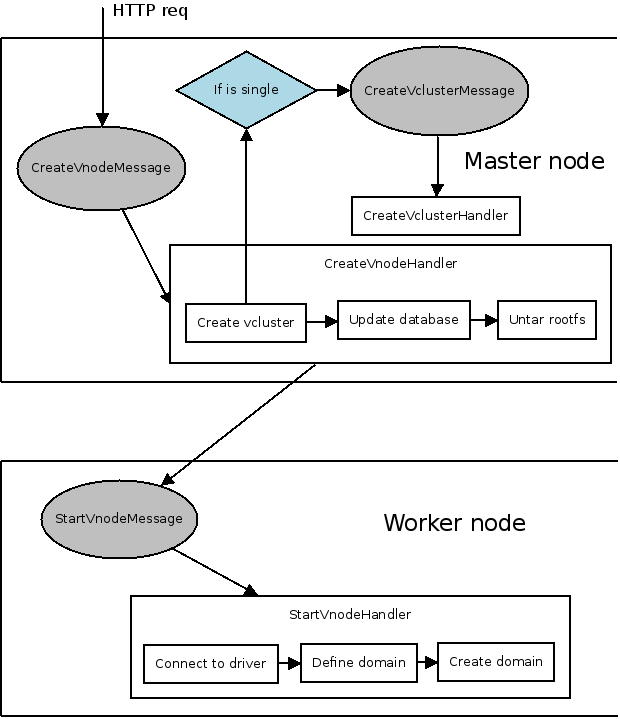
\includegraphics[width=0.9\textwidth]{create-vnode}
    \caption{创建虚拟容器的工作流程}
\end{figure}

虽然 Tsinghua NOVA 系统会通过 RPC 通知相应的从节点新的虚拟容器应该被创建,但是解压缩
根文件系统这个步骤是在主节点操作的。这是基于两个事实:一是我们的系统里运行 web 界面服务的
HTTP server 是跑在主节点上的,也就是说,用户在网页端发出在某个宿主机上“新建虚拟容器”
这个 HTTP 请求之后,主节点不通过任何 RPC 就可以收到这个 HTTP 请求;二是如果在从节点上
运行的 Tsinghua NOVA 守护进程上做根文件系统的解压缩,那么就会产生大量的网络 I/O ,
因为从节点上挂载的 NFS 目录必须和主节点保持同步,而我们的测试集群使用的是千兆以太网,相对
于万转的机械硬盘,以太网的吞吐率 (throughput) 是很低的,所以容易成为瓶颈。

\begin{figure}[H]
    \centering
    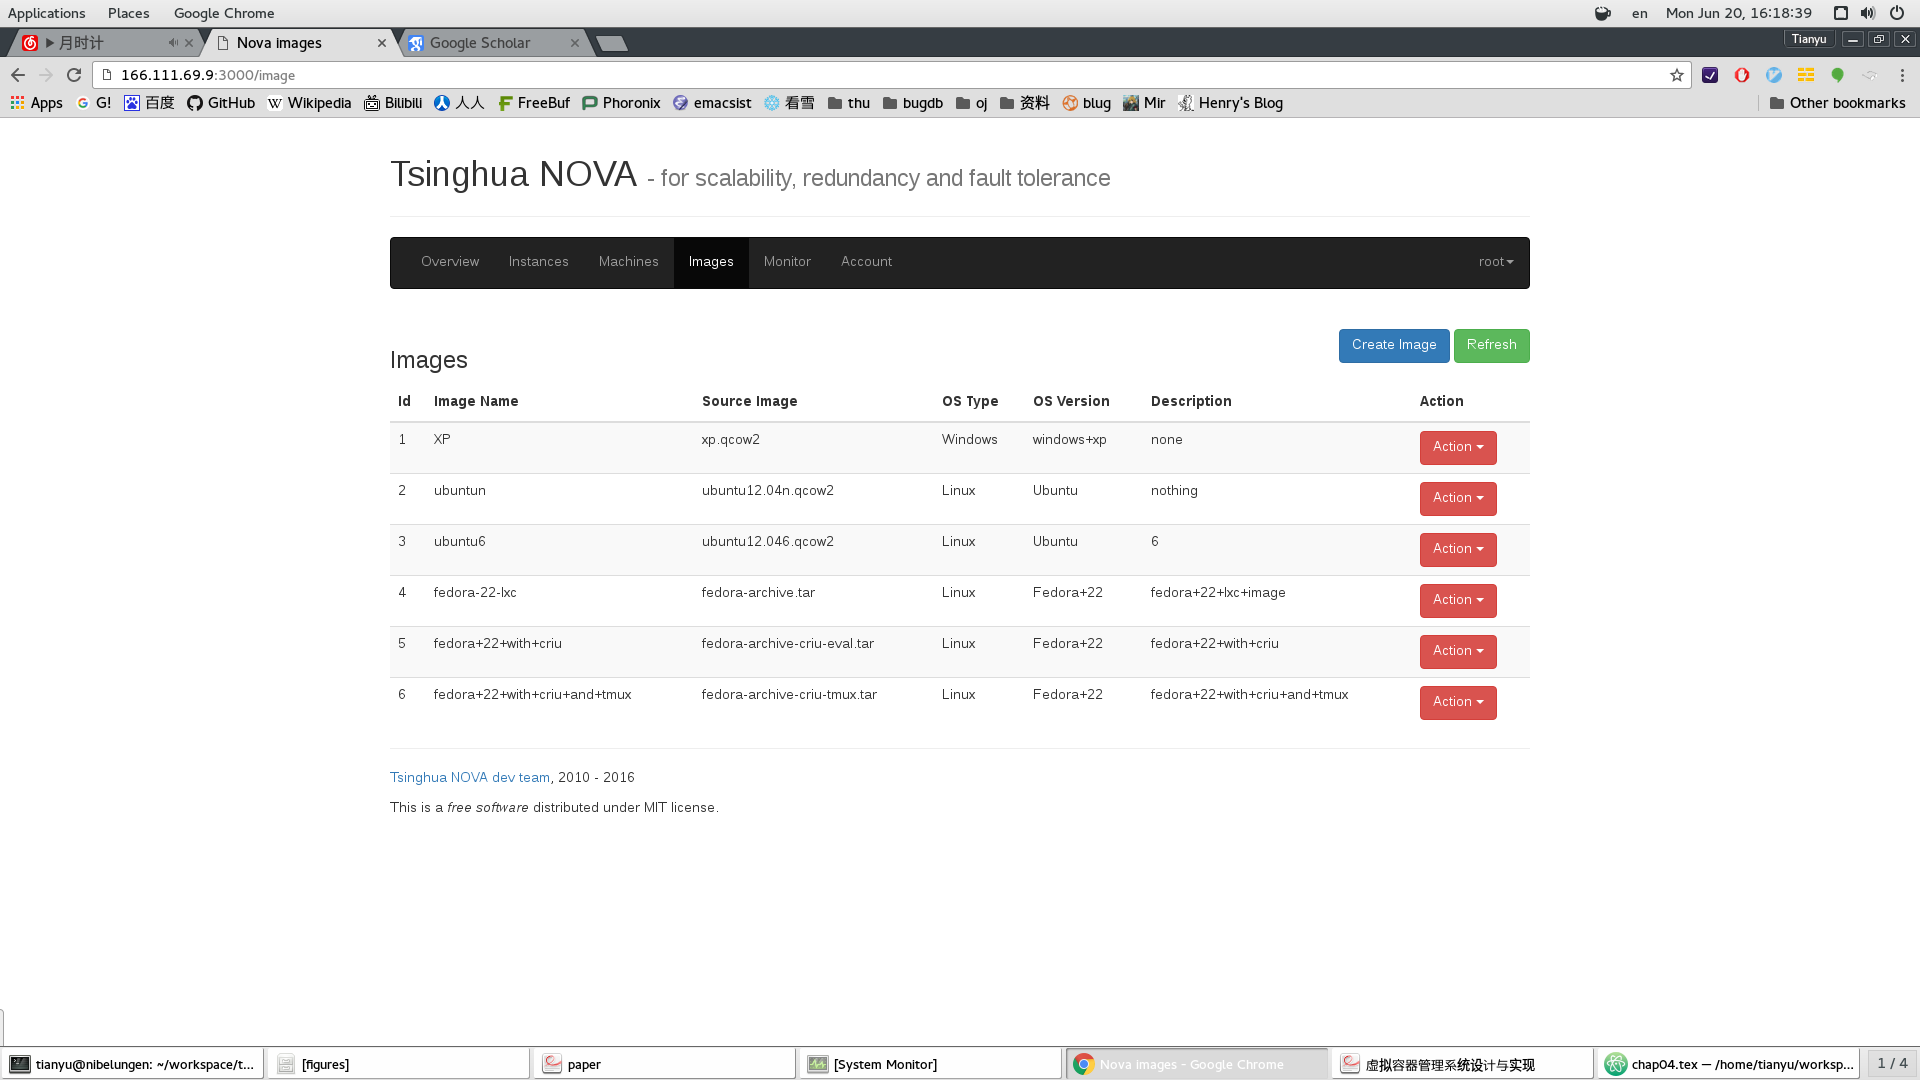
\includegraphics[width=0.7\textwidth]{image-manager}
    \caption{Tsinghua NOVA 的镜像管理界面}
\end{figure}

在这个系统中,容器的基镜像被存储在 \$NOVA\_HOME/run/run 目录,这个目录是从主节点上的某个
目录\footnote{例如在我们的测试系统中是 /home/export,但是这个没有关系}挂载过来的,无论
主节点从节点都是如此,我们称被挂载的目录为 NFS 基目录 (NFS base directory) 。而每个
运行着的虚拟容器都保存着一份自己独立的文件系统,在容器部署之初,是由相应的基文件系统的压缩包
直接解压过来的。同时,在每个容器自己的目录下还保存着一个 XML 文件包含了一些资源的定义,这个
文件将在下一节详细介绍。例如名字是 testlxc 的虚拟容器它的目录就是 \$NOVA\_HOME/run/run/
testlxc ,里面包含一个 conf.xml 文件和一个 rootfs/ 目录。

\begin{lstlisting}
testlxc
|-- conf.xml
|-- rootfs/

1 directory, 1 file
\end{lstlisting}

\subsubsection{XML 配置文件的定义}
\label{subsubsec:xml-definition}

在 ~\ref{subsubsec:deployment-rootfs} 小节提到,需要对 Linux 虚拟容器定义一个配置文件
conf.xml ,在这一小节,具体讲解这个配置文件的来龙去脉。

\begin{figure}[h]
    \centering
    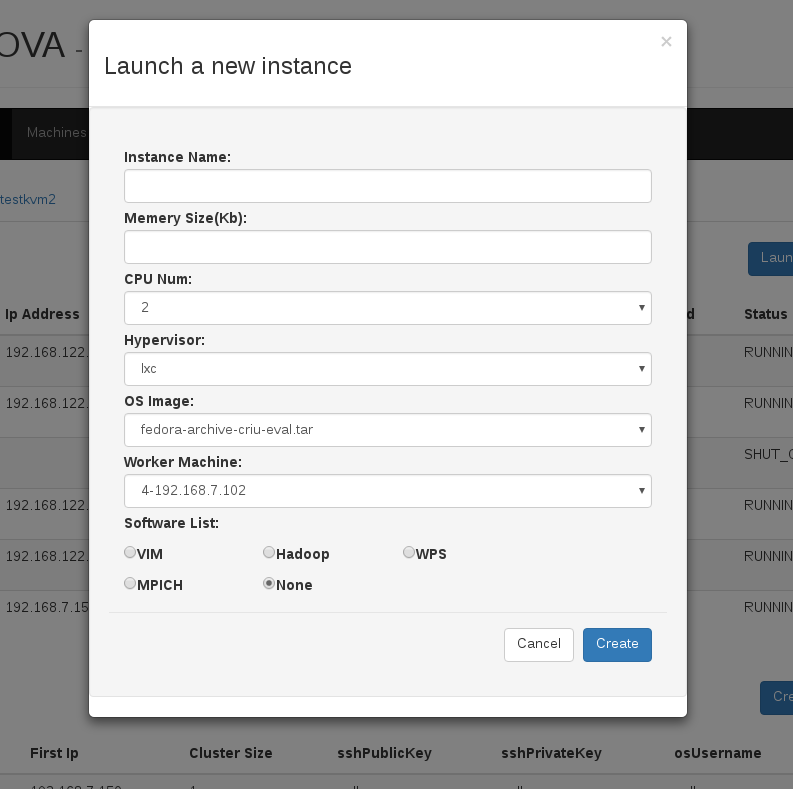
\includegraphics[width=0.4\textwidth]{guest-config-dialog}
    \caption{客户虚拟机配置界面}
\end{figure}

首先要强调,这个配置文件是使用 libvirt 管理 LXC 所需要的,如果使用 LXC 自己的用户态工具,
那么需要使用另外格式的配置文件定义,而两者可以使用 libvirt 提供的工具 domxml-from-native
进行转换,例如转换一个叫做 testlxc 的虚拟容器的 config 文件:

\begin{lstlisting}
virsh -c lxc:/// domxml-from-native lxc-tools /var/lib/lxc/testlxc/config
\end{lstlisting}

一个简单的例子:

\begin{lstlisting}
    <domain type='lxc'>
      <name>testlxc</name>
      <uuid>cd7aedef-a0f6-470e-923c-64275b437937</uuid>
      <memory unit='KiB'>512000</memory>
      <currentMemory unit='KiB'>512000</currentMemory>
      <vcpu placement='static'>1</vcpu>
      <resource>
        <partition>/machine</partition>
      </resource>
      <os>
        <type arch='x86_64'>exe</type>
        <init>/sbin/init</init>
      </os>
      <features>
        <capabilities policy='allow'>
        </capabilities>
      </features>
      <clock offset='utc'/>
      <on_poweroff>destroy</on_poweroff>
      <on_reboot>restart</on_reboot>
      <on_crash>destroy</on_crash>
      <devices>
        <emulator>/usr/libexec/libvirt_lxc</emulator>
        <filesystem type='mount' accessmode='passthrough'>
          <source dir='/home/Nova/run/run/testlxc/rootfs'/>
          <target dir='/'/>
        </filesystem>
        <interface type='bridge'>
          <mac address='fe:13:f4:44:1c:3'/>
          <source bridge='virbr0'/>
          <link state='up'/>
        </interface>
        <console type='pty'>
          <target type='lxc' port='0'/>
        </console>
      </devices>
    </domain>
\end{lstlisting}

从这个例子中,可以看出 XML 包含几个关键的属性:

\begin{enumerate}
    \item \textbf{domain type:} 这个域 (domain) \footnote{在 libvirt 里一个虚拟机
    称为一个域,域是 libvirt 管理的基本单位}的类型,如果是 LXC 就是 lxc ,如果是
    QEMU-KVM 就是 kvm ;
    \item \textbf{name:} 这个域的名称。在 Tsinghua NOVA 系统里,名称可以由用户
    在网页的对话框里指定;
    \item \textbf{uuid:} 是一个域的通用唯一识别码。在 Tsinghua NOVA 里是自动生成的;
    \item \textbf{memory:} 对虚拟机内存的限制;具体到我们关心的 LXC 来说,就是通过
    ~\ref{subsubsec:cgroup}小节提到的 cgroup 控制组技术限制运行在虚拟容器中的进程组
    的最大内存配额,达到资源限制的作用;
    \item \textbf{vcpu:} 和 \textbf{memory} 类似,通过控制 cgroup 的 cpuset 参数
    达到限制 CPU 数量的目的。Intel 的超线程 (Hyperthreading) 技术可以使处理器的物理
    核心数翻倍,在这里会有一定的优势;
    \item \textbf{source:} 虚拟机的磁盘镜像或者根文件系统的绝对路径。
\end{enumerate}

\subsection{对虚拟机管理程序的抽象}

Tsinghua NOVA 平台在设计的时候,一个很重要的特性就是对虚拟机管理程序 (hypervisor) 的
抽象。在代码中,这一点主要体现在 worker.nova.worker.virt 这个包。

目前 Tsinghua NOVA 只对两种虚拟机管理程序\footnote{Xen on libvirt 的条件判断在很多
文件中写了,但这不代表 NOVA 已经支持了 Xen ,实际上还有很多工作要做}\footnote{LXC 严格
来说不算 hypervisor ,有人提出了 lightervisor 的这种说法}——QEMU-KVM 和 LXC 。相应
的代码在上述包中的 Lxc.java 和 Kvm.java 两个类里。

比较关键的方法一个是生成 MAC 地址的 generateMacAddr 和生成配置文件的 emitDomain 。
之所以要生成 MAC 地址是因为虚拟机使用的虚拟网卡需要一个 MAC 硬件地址。在下面的章节我们
会看到这个是非常关键的,因为和 libvirt 管理的虚拟网关的 DHCP 配置有关系。

在代码中的其它很多地方会看到对虚拟机管理程序的条件判断,这是因为目前对于虚拟机管理软件的
抽象还不够彻底。实际上,在本文作者成为 Tsinghua NOVA 的主要开发者以前,Tsinghua NOVA
甚至没有支持更多虚拟机管理软件的计划。

\section{虚拟容器的迁移}

这一节主要介绍如何在 Tsinghua NOVA 平台中实现了一个简单的容器实时迁移 (live migration)
系统。

首先要搞清楚为什么要实现迁移 (migration) 或者实时迁移 (live migration) 。我们在前文
提到,一个虚拟集群中需要通过迁移进行调度。所谓实时迁移,就是在迁移过程中一方面尽量减小服务的
宕机时间 (downtime) ,使得服务尽可能随时可用;另一方面保存迁移前服务的状态,不至于使得
服务“从头再来”。比如说客户虚拟机运行的服务是使用 mplayer 播放的一首歌曲,那么迁移前播放到
哪个位置,迁移之后还要从那个位置开始播放。

当然,目前 Tsinghua NOVA 平台作为一个虚拟化管理系统,在迁移时不能保证完全没有开销。这
主要是因为 Tsinghua NOVA 是完全没有 replica 的。实现同一服务在不同物理节点之间的
状态复制 (state machine replication) 和容灾恢复,可以使用 Paxos 协议进行状态同步,
其中一个对上层服务透明的系统是哥伦比亚大学的 Crane 系统~\cite{cui2015p}。

\subsection{LXC 的迁移和 QEMU-KVM 的迁移的区别}

\begin{figure}[h]
    \centering
    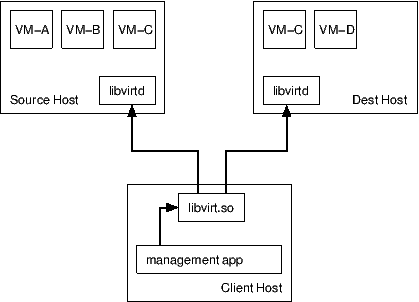
\includegraphics[width=0.6\textwidth]{migration-managed-direct}
    \caption{Libvirt managed direct migration}
\end{figure}

LXC 和 KVM 的迁移的主要区别是到目前为止 libvirt 没有一个较好的对 LXC 的原生迁移 (native
 migration) 的实现,而这一点对于 KVM 是有的。这也让 KVM 的迁移实现起来毫无难度。

在命令行下使用 libvirt 的 shell 工具 virsh 进行迁移的实例如下,其中 test-migrate 是
客户虚拟机的名字、desthost 是目标宿主机的主机名 (hostname) :

\begin{lstlisting}
# kvm guest
virsh migrate test-migrate qemu+ssh://desthost/system
# xen guest
virsh migrate test-migrate xen+tls://desthost/system
\end{lstlisting}

\subsection{实现非实时迁移}

\begin{algorithm}[H]
    \begin{algorithmic}
    \If {$hypervisor = lxc$}
        \State $xml\gets srcDomain.getXml()$
        \If {$srcDomain.active = 1$}
            \State $srcDomain.destroy()$
        \EndIf
        \State $srcDomain.undefine()$
        \State $dstDomain.define(xml)$
        \State $dstDomain.create()$
    \EndIf
    \end{algorithmic}
    \caption{非实时迁移的实现}
\end{algorithm}

简单来说,虚拟容器的迁移就是暂存客户虚拟容器的配置信息、关闭要迁移的客户虚拟容器、
从源宿主机取消域定义、在目标宿主机上重新按照暂存的 XML 配置信息定义域、最后重新在新的宿主
上启动这个域也就是要迁移的客户虚拟容器的过程。因为这些操作提供的 Java API 都是阻塞的,一个
返回了之后才会继续执行下一个,所以无须使线程休眠。需要注意的是,在关闭虚拟容器时使用的是
destroy() 方法而不是一般的 shutdown() ,主要是考虑到后者是非阻塞的,因为需要一段时间
等待客户机的内核关闭。

\subsection{实现实时迁移}

所谓的实时迁移在这里指的就是保存了服务状态的迁移过程,这一小节主要解释如何使用开源的
checkpoint/restore (C/R) 程序实现服务状态的迁移。

需要注意,实时迁移和完全没有宕机时间 (downtime) 的迁移还不尽相同,后者一般称为
seamless live migration ,因为它的开销小到不至于被终端用户 (end-user) 察觉。

\subsubsection{在虚拟容器中配置 criu}

在 ~\ref{subsubsec:deployment-rootfs} 小节中,提到了虚拟容器的文件系统在迁移过程中是
保持静态的,也就是迁移的只是配置信息而不是整个根文件系统 (rootfs) 。这样,如果在迁移之前
就将负载的关键进程的内存状态等信息 dump 进文件系统,然后迁移之后再从相应的文件里恢复,
就可以实现负载的实时迁移了。

上述功能是使用开源 C/R 工具 criu 实现的,顾名思义,就是“用户态的 C/R 工具”的意思。
在使用最小安装的 Fedora 操作系统的容器中编译安装 criu 的方法如下:

\begin{lstlisting}[language=bash]
cd ~; git clone https://github.com/xemul/criu
cd criu; make
\end{lstlisting}

\subsubsection{安装 libvirt 的驱动}

想要通过 libvirt 对 Linux 虚拟容器进行操作,就要安装相应的驱动 (driver) 。以下的命令
可以在 CentOS 7 上使用默认的包管理器 rpm 和 yum 安装 LXC 和 libvirt 驱动等依赖:

\begin{lstlisting}[language=bash]
# download EPEL package
wget https://dl.fedoraproject.org/pub/epel/epel-release-latest-7.noarch.rpm
# with ROOT
# installs EPEL package first
rpm -ivh epel-release-latest-7.noarch.rpm
# installs lxc and templates
yum install lxc lxc-templates lxc-libs
# installs libvirt drivers
yum install libvirt-daemon-driver-lxc libvirt-daemon-lxc
\end{lstlisting}

\subsubsection{C/R 自动化脚本}
\label{subsubsec:cr-automation}

这个脚本是用来在用户态对关键服务的进程进行 C/R 使用的,有如下几个参数:

\begin{enumerate}
    \item \textbf{checkpoint | restore} 选择是进行保存进程现场还是恢复现场;
    \item \textbf{-c | --container} 用于指定虚拟容器的名称。如果 --ipaddr 参数
    没有提供的话,将调用 nova-vmaddrctl 工具在 ARP 表缓存中寻找容器对应的 IP 地址;
    \item \textbf{-p | --process} 用于指定关键服务的进程名称。即使服务拥有多个进程
    ,比如 Apache httpd ,也可以正常工作。脚本按照进程名称查找对应的 PID ;
    \item \textbf{-i | --ipaddr} 如果这个参数被设置,那么 --container 就无效。这个
    参数是用来明文指定虚拟容器的 IP 地址的。
\end{enumerate}

其中,nova-vmaddrctl 的实现方式是首先从域的 XML 配置定义中读取虚拟网卡的 MAC 地址,再
在宿主机的 ARP 表缓存中寻找虚拟容器对应的 IP 地址。这个脚本的有效性和 ARP 缓存的超时时间
(timeout) 设置有关。

通过阅读 criu 的代码,发现 criu 要求 /proc/sys/kernel/ns\_last\_pid 的写权限。但是
容器默认的 procfs 被挂载为只读,所以 C/R 脚本会自动检查 ns\_last\_pid 的可写性,如果
发现是只读的,那么就需要重新挂载 procfs :

\begin{lstlisting}[language=bash]
mount -o remount,rw /proc/sys
\end{lstlisting}

实际上 criu 自带的一个参数 check 可以协助检查相关的设置是否满足 criu 正常运行的要求。

在使用 criu 的时候,加入了参数 --shell-job ,那么需要有一个 tty 才能正常工作。
在 C/R 脚本中,使用 Tmux 开启了一个伪终端,然后将 criu 需要的按键序列使用 Tmux 发送
进虚拟容器内的操作系统。

需要注意的是,如果使用 ssh 连进虚拟容器也会在 /dev/pts 下产生一个伪终端设备,而保存、
恢复现场,也就是 checkpoint/restore 的过程中,/dev/pts 下的伪终端设备必须保持完全
相同才可以。如果恢复进程失败了,那么有很大的可能性是环境中增加或减少了设备。

\subsubsection{配置 libvirt DHCP}

如果因为实验环境的需要,始终要保持 ARP 缓存为热 (warm cache) 的,可以在宿主机上插入静态的
ARP 缓存表项目:

\begin{lstlisting}[language=bash]
arp -s 192.168.122.4 fe:13:6d:74:d6:a3
\end{lstlisting}

查看:

\begin{lstlisting}[language=bash]
# Linux mode
arp -e
# BSD mode
arp -a
\end{lstlisting}

删除 IP 地址对应的表项:

\begin{lstlisting}[language=bash]
arp -d 192.168.122.4
\end{lstlisting}

在 virsh 命令行下,可以修改 libvirt 虚拟网络的 DHCP 服务设置,从而绑定静态的 IP 地址。

查看所有 libvirt 网络配置:

\begin{lstlisting}
net-list
\end{lstlisting}

查看 default 网络的配置信息:

\begin{lstlisting}
net-dumpxml default
\end{lstlisting}

XML 格式的输出:

\begin{lstlisting}
    <network>
      <name>default</name>
      <uuid>666bb0b0-1760-4507-a41f-2d15bd27af3a</uuid>
      <forward mode='nat'>
        <nat>
          <port start='1024' end='65535'/>
        </nat>
      </forward>
      <bridge name='virbr0' stp='on' delay='0'/>
      <mac address='52:54:00:b1:d0:62'/>
      <ip address='192.168.122.1' netmask='255.255.255.0'>
        <dhcp>
          <range start='192.168.122.2' end='192.168.122.254'/>
        </dhcp>
      </ip>
    </network>
\end{lstlisting}

修改 default 的配置:

\begin{lstlisting}
net-edit default
\end{lstlisting}

修改后的配置:

\begin{lstlisting}
    <network>
      <name>default</name>
      <uuid>666bb0b0-1760-4507-a41f-2d15bd27af3a</uuid>
      <forward mode='nat'>
        <nat>
          <port start='1024' end='65535'/>
        </nat>
      </forward>
      <bridge name='virbr0' stp='on' delay='0'/>
      <mac address='52:54:00:b1:d0:62'/>
      <ip address='192.168.122.1' netmask='255.255.255.0'>
        <dhcp>
          <range start='192.168.122.100' end='192.168.122.254'/>
          <host mac='fe:13:6d:74:d6:a3' ip='192.168.122.4'/>
          <host mac='fe:13:86:d8:c8:92' ip='192.168.122.5'/>
        </dhcp>
      </ip>
    </network>
\end{lstlisting}

重启网络:

\begin{lstlisting}
net-destroy default
net-start default
\end{lstlisting}

\subsubsection{实时迁移}

实时迁移只需要在非实时迁移的代码基础上增加 C/R 的过程就可以了。对于目标主机,既可以使用
Tsinghua NOVA 提供的 RPC 机制,也可以使用 ssh 。

修改后的伪代码如下:

\begin{algorithm}[H]
    \begin{algorithmic}
    \If {$hypervisor = lxc$}
        \State $checkpoint()$
        \State $xml\gets srcDomain.getXml()$
        \If {$srcDomain.active = 1$}
            \State $srcDomain.destroy()$
        \EndIf
        \State $srcDomain.undefine()$
        \State $dstDomain.define(xml)$
        \State $dstDomain.create()$
        \State $restore()$
    \EndIf
    \end{algorithmic}
    \caption{实时迁移的实现}
\end{algorithm}

\subsection{迁移类型的配置}

在 Tsinghua NOVA 中,通过 *.properties 文件可以很方便地为各项参数进行配置,迁移也不例外。
使用 \$NOVA\_HOME/conf/nova.lxc-cr.properties 可以对 LXC 迁移进行配置:

\begin{lstlisting}
######################################
# the lxc checkpoint/restore section #
######################################

# the name of the payload process
payload_process.name=toy.py
# migration type: 'live' or 'offline'
migration_type=offline
# username of the container
username=root
# password
passwd=940715
\end{lstlisting}

其中,payload\_process.name 是容器中负载应用程序的进程名字,migration\_type 选择是否是
实时迁移,username 和 passwd 是虚拟容器的用户名密码。

\section{实时获取准确的虚拟机 IP 地址}

原先 Tsinghua NOVA 系统的虚拟机 IP 地址是从主节点运行的数据库服务上获得的,而且这个 IP
是在虚拟机创建的时候以静态的形式分配的,非常死板。通过为 VnodeStatusDaemon 打补丁,支持
了虚拟机节点的 IP 地址实时获取。

\begin{figure}[h]
    \centering
    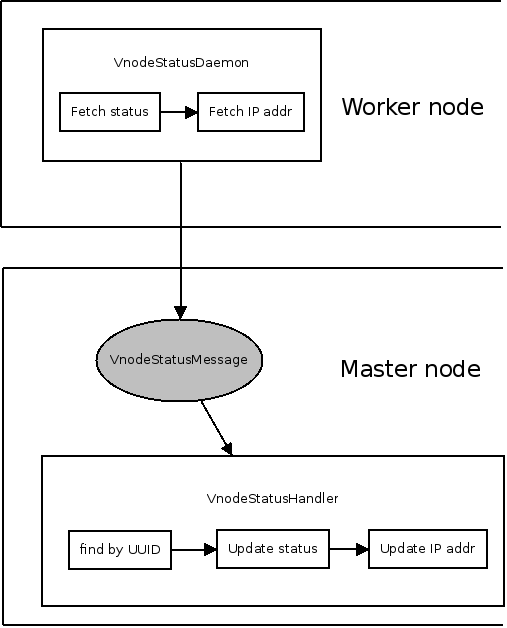
\includegraphics[width=0.8\textwidth]{vnode-status}
    \caption{获取虚拟机状态的基本流程}
\end{figure}

原理还是使用~\ref{subsubsec:cr-automation}小节介绍的 nova-vmaddrctl 脚本从 ARP 缓存中读取 IP
地址。然后采用 RPC 的方式传回主节点更新数据库中的虚拟节点信息。
